% CS615 Aspects of System Administration
% Author: Jan Schaumann <jschauma@netmeister.org>

\documentclass[xga]{xdvislides}
\usepackage[landscape]{geometry}
\usepackage{graphics}
\usepackage{graphicx}
\usepackage{colordvi}

\newcommand{\smallish}{\fontsize{18}{18}\selectfont}

\begin{document}
\setfontphv

%%% Headers and footers
\lhead{\slidetitle}				% default:\lhead{\slidetitle}
\chead{CS615 - Aspects of System Administration}% default:\chead{\relax}
\rhead{Slide \thepage}				% default:\rhead{\sectiontitle}
\lfoot{\Gray{Lecture 01: Introduction}}		% default:\lfoot{\slideauthor}
\cfoot{\relax}					% default:\cfoot{\relax}
\rfoot{\Gray{\today}}

\vspace*{\fill}
\begin{center}
	\Hugesize
		CS615 - Aspects of System Administration\\ [1em]
	\hspace*{5mm}\blueline\\ [1em]
	\Normalsize
		Department of Computer Science\\
		Stevens Institute of Technology\\
		Jan Schaumann\\
		\verb+jschauma@stevens.edu+ \\
		\verb+https://www.cs.stevens.edu/~jschauma/615/+
\end{center}
\vspace*{\fill}

\subsection{New Rules}
\Hugesize
\vspace*{\fill}
\begin{center}
Close your laptops! (Silence phones etc.)
\end{center}
\vspace*{\fill}
\Normalsize

\subsection{New Rules}
\Hugesize
\vspace*{\fill}
\begin{center}
Close your laptops! (Silence phones etc.) \\
\vspace{.5in}
Open your eyes! \\
\small
(Mind, too.)
\end{center}
\vspace*{\fill}
\Normalsize

\subsection{A rose by any other name...}
\vspace*{\fill}
\begin{center}
	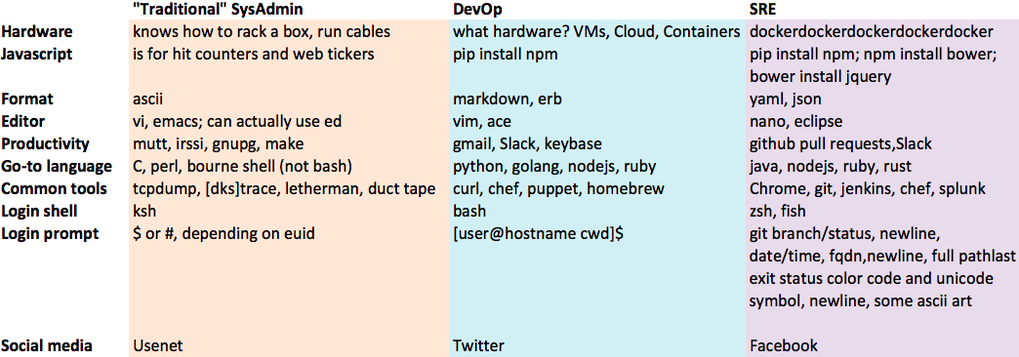
\includegraphics[scale=0.6]{pics/sysadmin-personalities.eps} \\
\end{center}
\vspace*{\fill}

\subsection{How we see ourselves}
\vspace*{\fill}
\begin{center}
	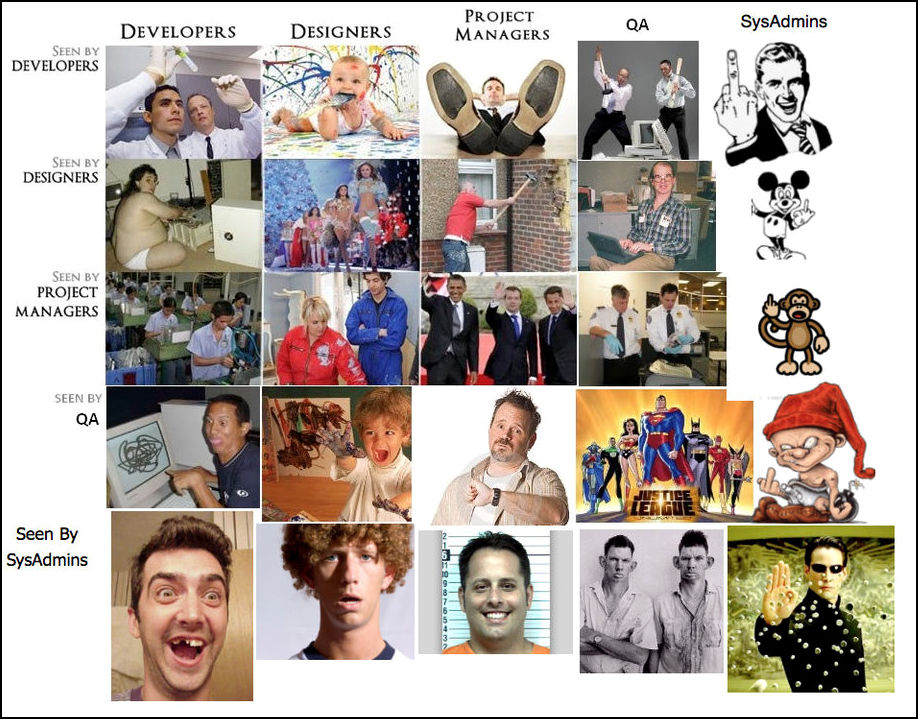
\includegraphics[scale=0.45]{pics/as-seen-by.eps} \\
\end{center}
\vspace*{\fill}

\subsection{The Job of a System Administrator}
What {\bf exactly} does a {\em System Administrator} do?

\subsection{The Job of a System Administrator}
What {\bf exactly} does a {\em System Administrator} do?
\vspace*{\fill}
\begin{center}
	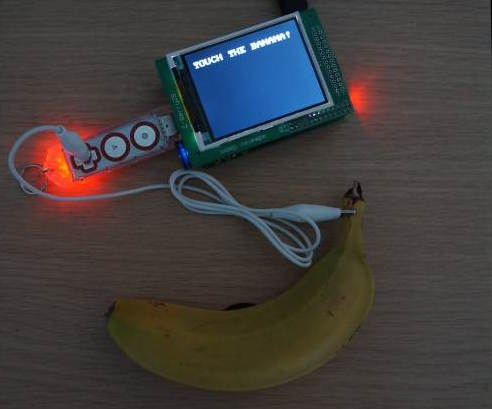
\includegraphics[scale=0.7]{pics/banana-wifi.eps} \\
\end{center}
\vspace*{\fill}
{\tt https://is.gd/8vKPhl}

\subsection{The Job of a System Administrator}
\begin{center}
	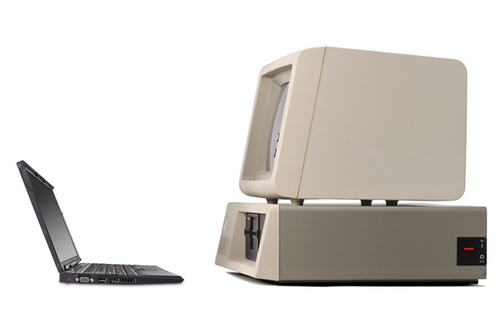
\includegraphics[scale=0.9]{pics/computers.eps} \\
\end{center}

\subsection{The Job of a System Administrator}
\vspace*{\fill}
\begin{center}
	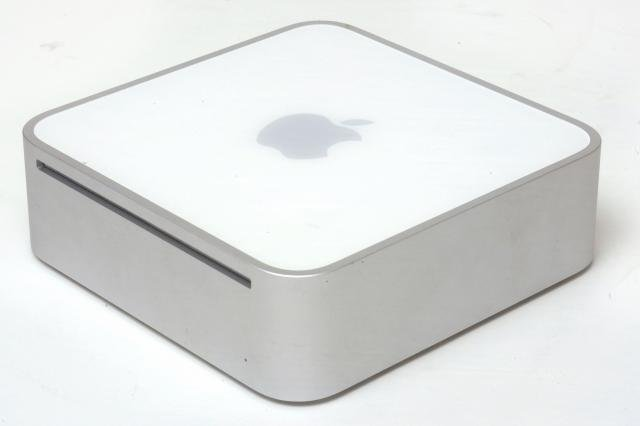
\includegraphics[scale=0.6]{pics/macmini.eps} \\
\end{center}
\vspace*{\fill}

\subsection{The Job of a System Administrator}
\vspace*{\fill}
\begin{center}
	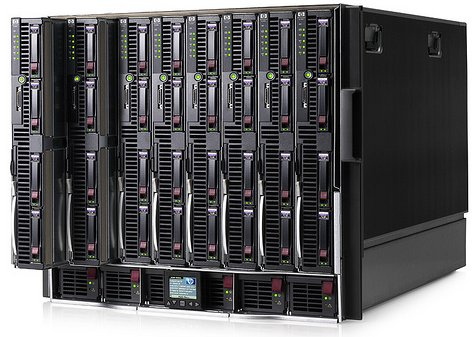
\includegraphics[scale=1.2]{pics/blades.eps} \\
\end{center}
\vspace*{\fill}

\subsection{The Job of a System Administrator}
\vspace*{\fill}
\begin{center}
	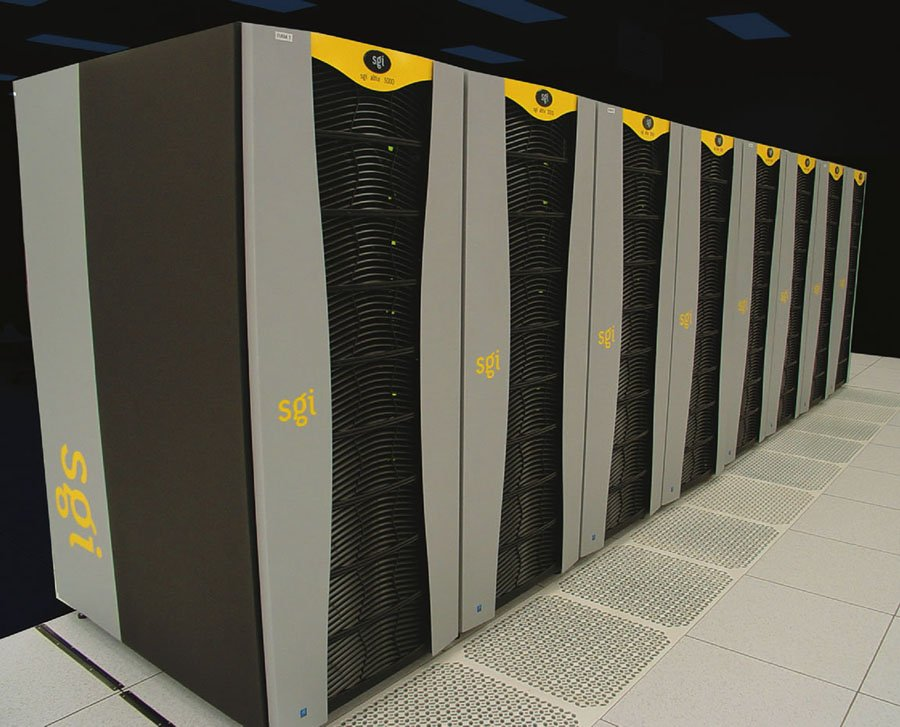
\includegraphics[scale=0.4]{pics/altix.eps} \\
\end{center}
\vspace*{\fill}

\subsection{The Job of a System Administrator}
\vspace*{\fill}
\begin{center}
	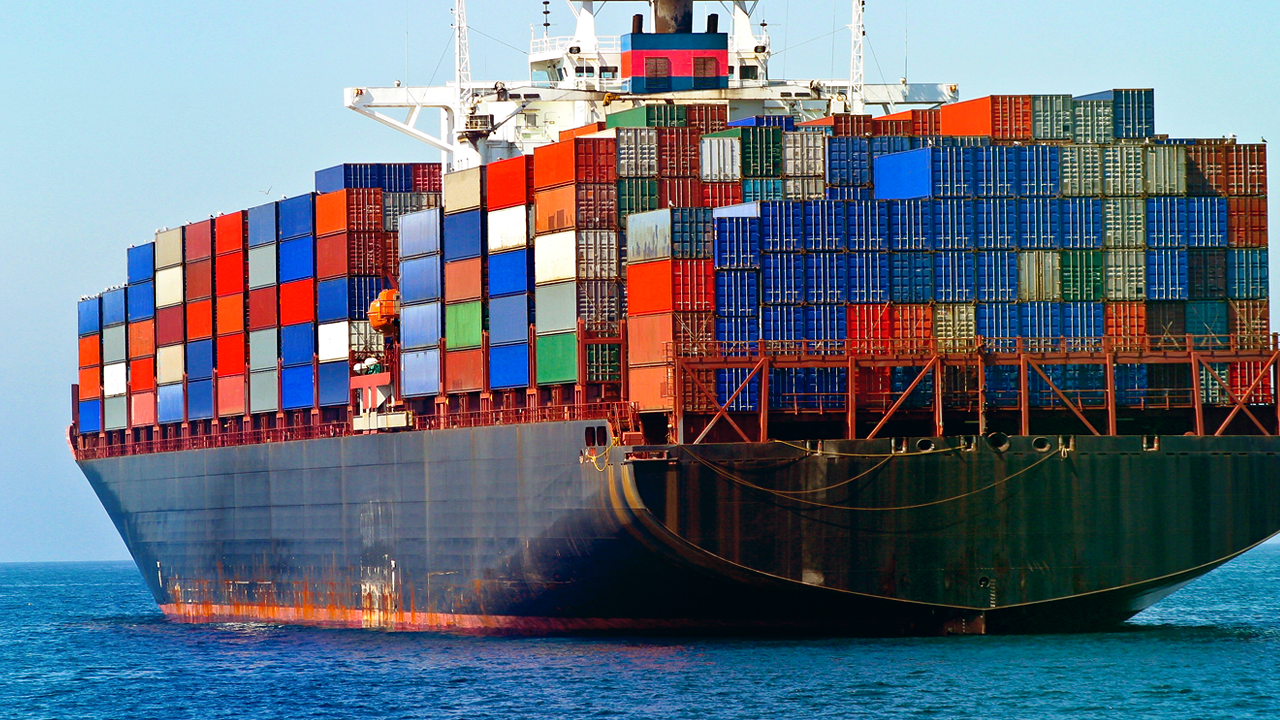
\includegraphics[scale=0.4]{pics/containers.eps} \\
\end{center}
\vspace*{\fill}

\subsection{The Job of a System Administrator}
\vspace*{\fill}
\begin{center}
	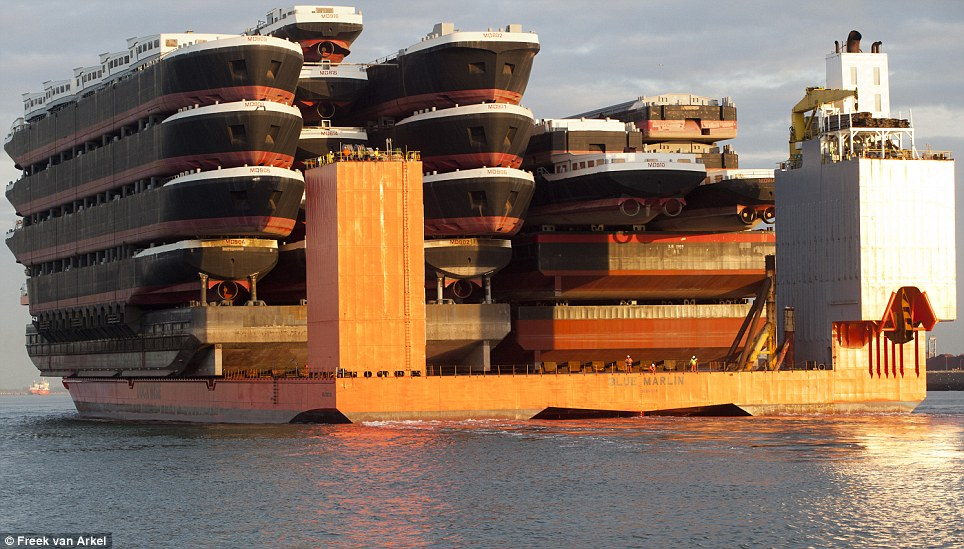
\includegraphics[scale=0.7]{pics/ship-shipping-ships.eps} \\
\end{center}
\vspace*{\fill}


\subsection{The Job of a System Administrator}
\vspace*{\fill}
\begin{center}
	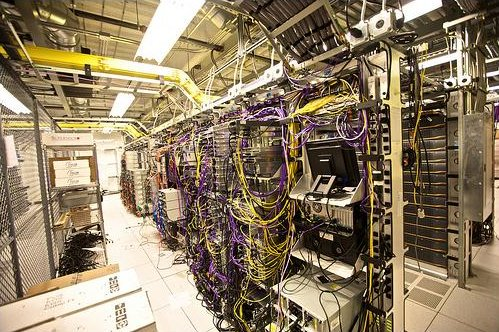
\includegraphics[scale=0.9]{pics/datacenter.eps} \\
\end{center}
\vspace*{\fill}

\subsection{The Job of a System Administrator}
\vspace*{\fill}
\begin{center}
	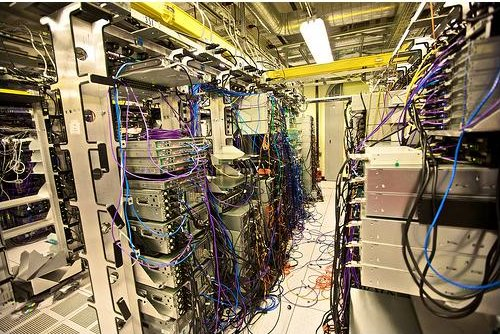
\includegraphics[scale=0.9]{pics/datacenter2.eps} \\
\end{center}
\vspace*{\fill}

\subsection{The Job of a System Administrator}
\vspace*{\fill}
\begin{center}
	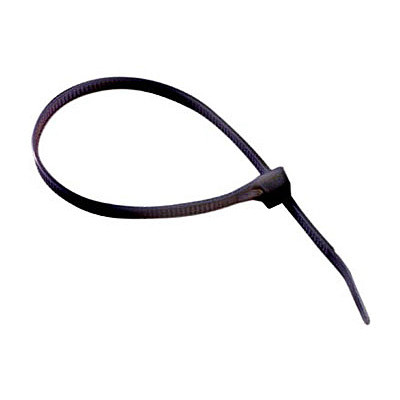
\includegraphics[scale=0.7]{pics/Cable_Tie.eps} \\
\end{center}
\vspace*{\fill}

\subsection{The Job of a System Administrator}
\vspace*{\fill}
\begin{center}
	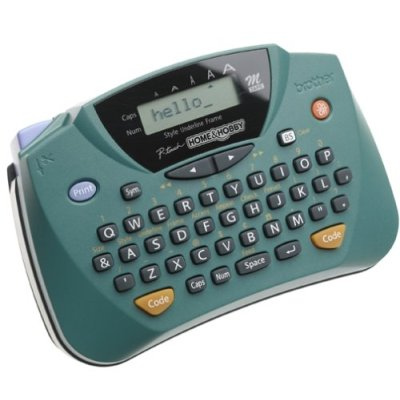
\includegraphics[scale=0.7]{pics/labelmaker.eps} \\
\end{center}
\vspace*{\fill}

\subsection{The Job of a System Administrator}
\vspace*{\fill}
\begin{center}
	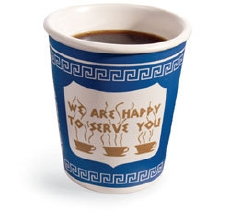
\includegraphics[scale=1.2]{pics/coffee.eps} \\
\end{center}
\vspace*{\fill}

\subsection{The Job of a System Administrator}
\vspace*{\fill}
\begin{center}
	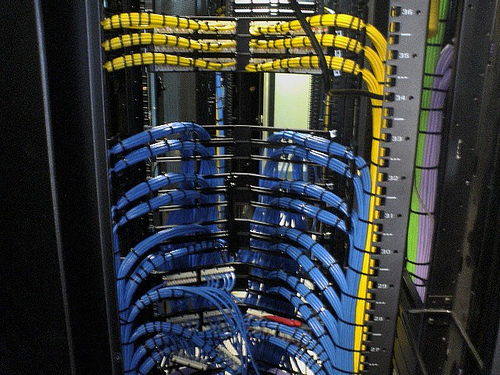
\includegraphics[scale=0.8]{pics/cables2.eps} \\
\end{center}
\vspace*{\fill}

\subsection{The Job of a System Administrator}
\vspace*{\fill}
\begin{center}
	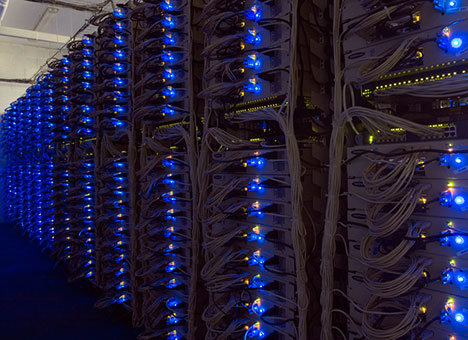
\includegraphics[scale=1.2]{pics/data-center-servers-t001.eps} \\
\end{center}
\vspace*{\fill}

\subsection{The Job of a System Administrator}
\vspace*{\fill}
\begin{center}
	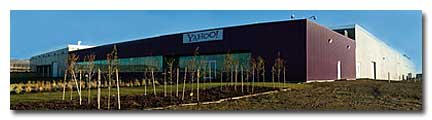
\includegraphics[scale=2.0]{pics/quincy-panorama.eps} \\
\end{center}
\vspace*{\fill}

\subsection{The Job of a System Administrator}
\vspace*{\fill}
\begin{center}
	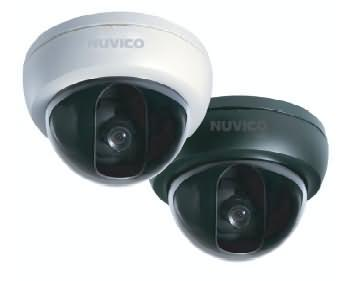
\includegraphics[scale=0.9]{pics/camera.eps} \\
\end{center}
\vspace*{\fill}

\subsection{The Job of a System Administrator}
\vspace*{\fill}
\begin{center}
	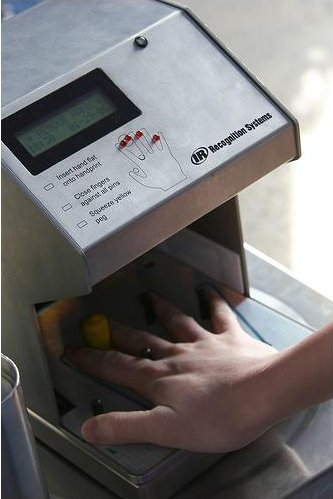
\includegraphics[scale=0.6]{pics/hand-scanner.eps} \\
\end{center}
\vspace*{\fill}

\subsection{The Job of a System Administrator}
\vspace*{\fill}
\begin{center}
	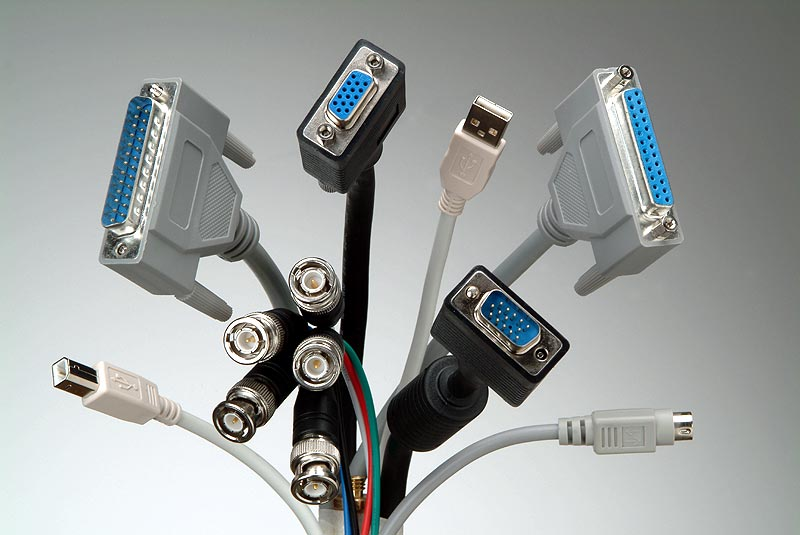
\includegraphics[scale=0.7]{pics/computer-cables-big.eps} \\
\end{center}
\vspace*{\fill}

\subsection{The Job of a System Administrator}
\vspace*{\fill}
\begin{center}
	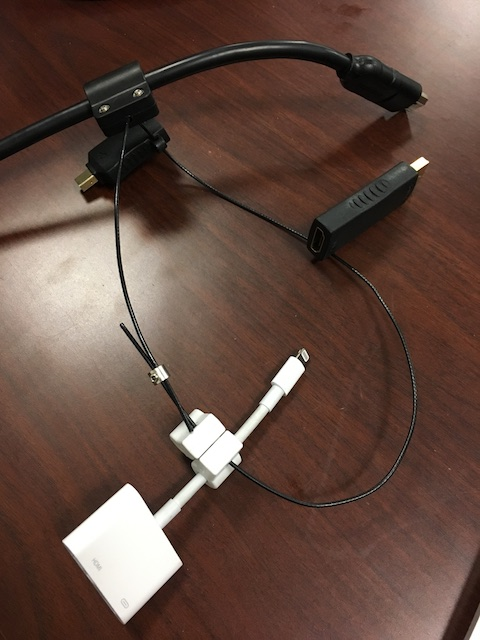
\includegraphics[scale=0.5]{pics/hdmi.eps} \\
\end{center}
\vspace*{\fill}


\subsection{The Job of a System Administrator}
\vspace*{\fill}
\begin{center}
	
\includegraphics[scale=0.5]{pics/wifi.eps} \\
\end{center}
\vspace*{\fill}

\subsection{The Job of a System Administrator}
\vspace*{\fill}
\begin{center}
	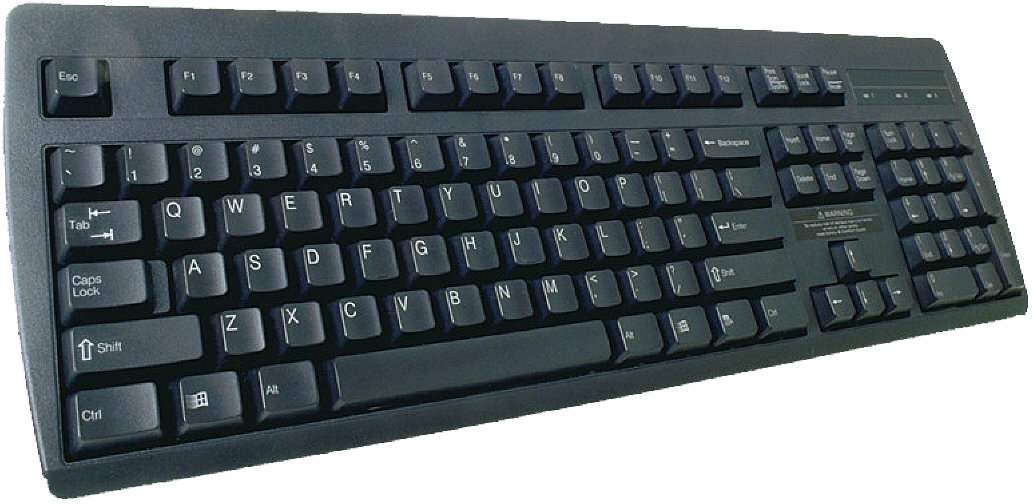
\includegraphics[scale=4.0]{pics/keyboard.eps} \\
\end{center}
\vspace*{\fill}

\subsection{The Job of a System Administrator}
\vspace*{\fill}
\begin{center}
	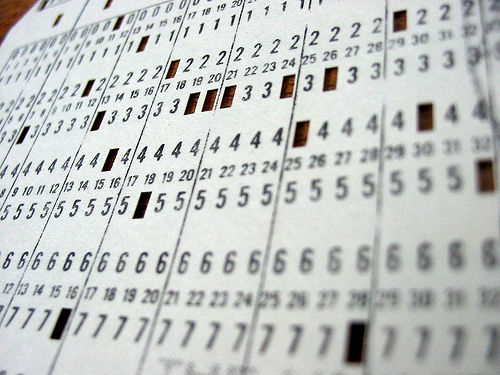
\includegraphics[scale=0.7]{pics/punchcard.eps} \\
\end{center}
\vspace*{\fill}

\subsection{The Job of a System Administrator}
\vspace*{\fill}
\begin{center}
	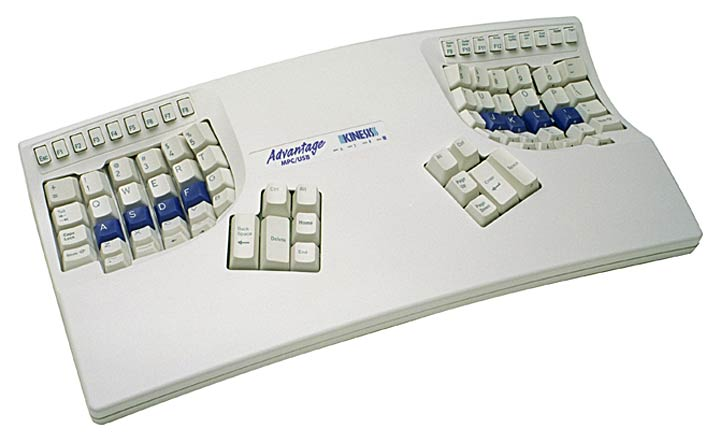
\includegraphics[scale=0.9]{pics/kinesis.eps} \\
\end{center}
\vspace*{\fill}

\subsection{The Job of a System Administrator}
\vspace*{\fill}
\begin{center}
	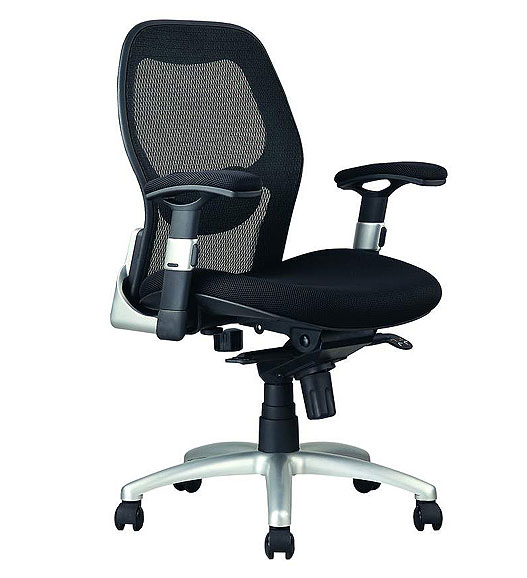
\includegraphics[scale=0.65]{pics/office-chair.eps} \\
\end{center}
\vspace*{\fill}

\subsection{The Job of a System Administrator}
\vspace*{\fill}
\begin{center}
	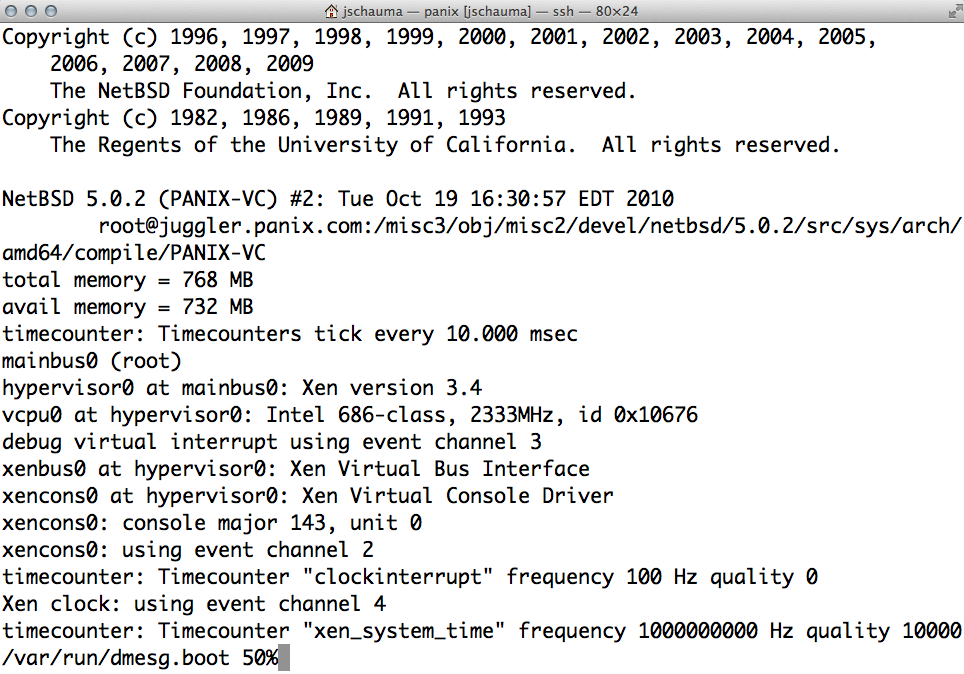
\includegraphics[scale=0.4]{pics/dmesg.eps} \\
\end{center}
\vspace*{\fill}

\subsection{The Job of a System Administrator}
\vspace*{\fill}
\begin{center}
	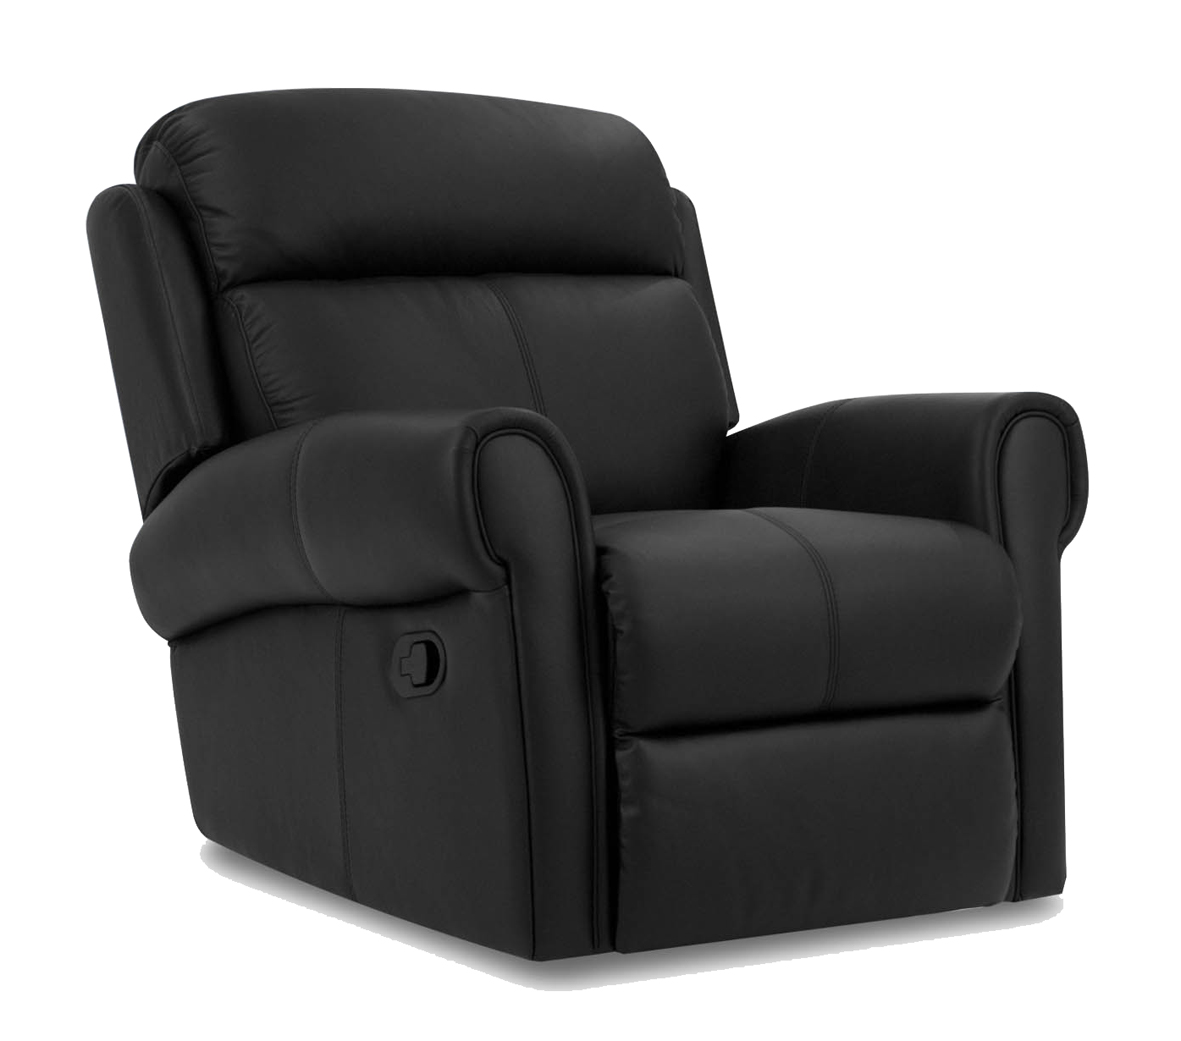
\includegraphics[scale=1.1]{pics/armchair.eps} \\
\end{center}
\vspace*{\fill}

\subsection{The Job of a System Administrator}
\vspace*{\fill}
\begin{center}
	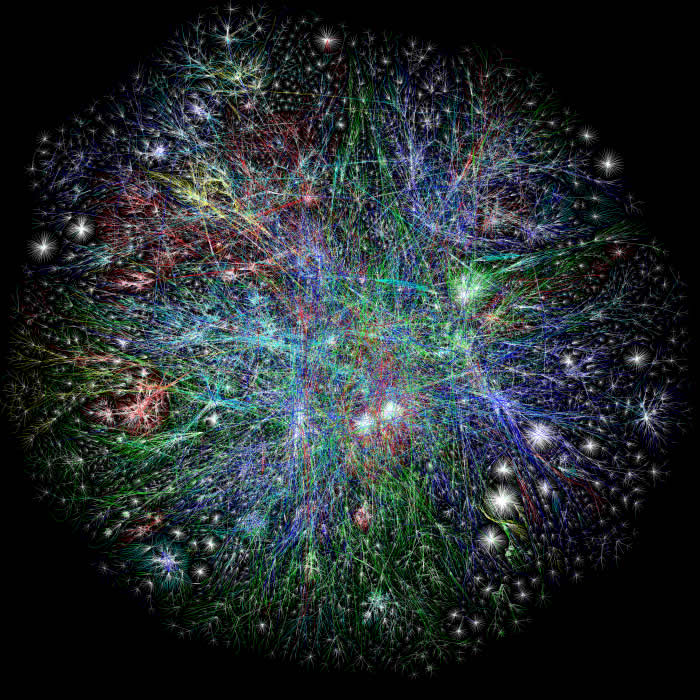
\includegraphics[scale=0.4]{pics/internet.eps} \\
	\small
	{\tt http://www.opte.org/maps/}
	\Normalsize
\end{center}
\vspace*{\fill}

\subsection{The Job of a System Administrator}
\vspace*{\fill}
\begin{center}
	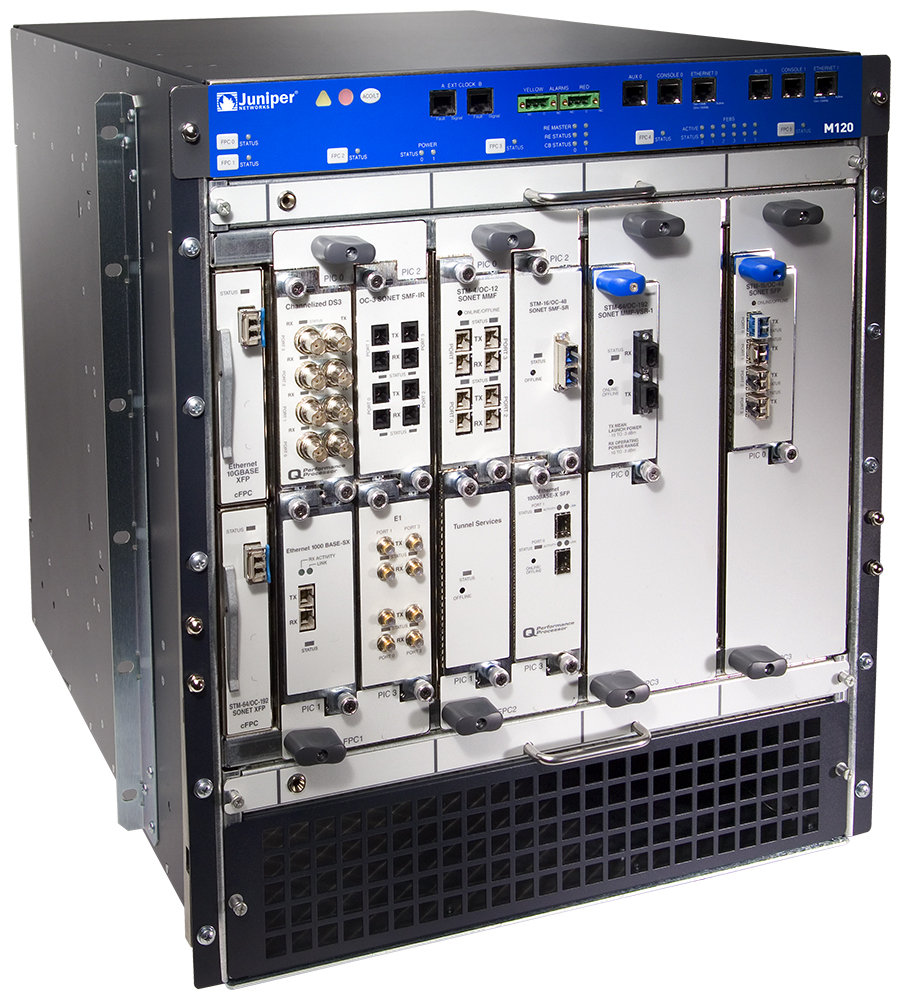
\includegraphics[scale=0.35]{pics/juniper.eps} \\
\end{center}
\vspace*{\fill}

\subsection{The Job of a System Administrator}
\vspace*{\fill}
\begin{center}
	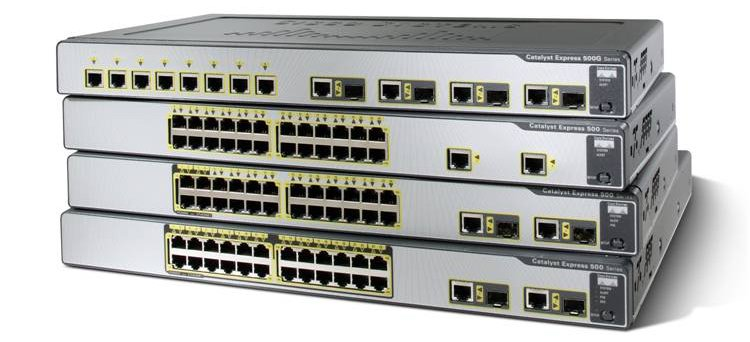
\includegraphics[scale=1.6]{pics/switches.eps} \\
\end{center}
\vspace*{\fill}

\subsection{The Job of a System Administrator}
\vspace*{\fill}
\begin{center}
	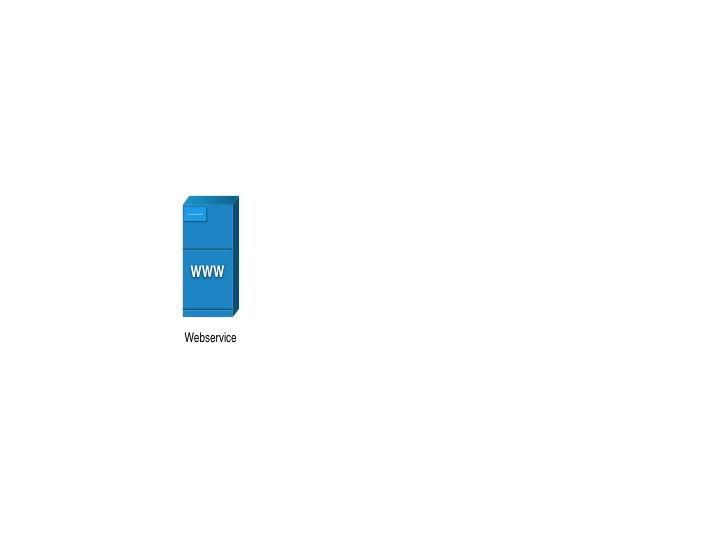
\includegraphics[scale=0.6]{pics/sample-infrastructure-0.eps} \\
\end{center}
\vspace*{\fill}

\subsection{The Job of a System Administrator}
\vspace*{\fill}
\begin{center}
	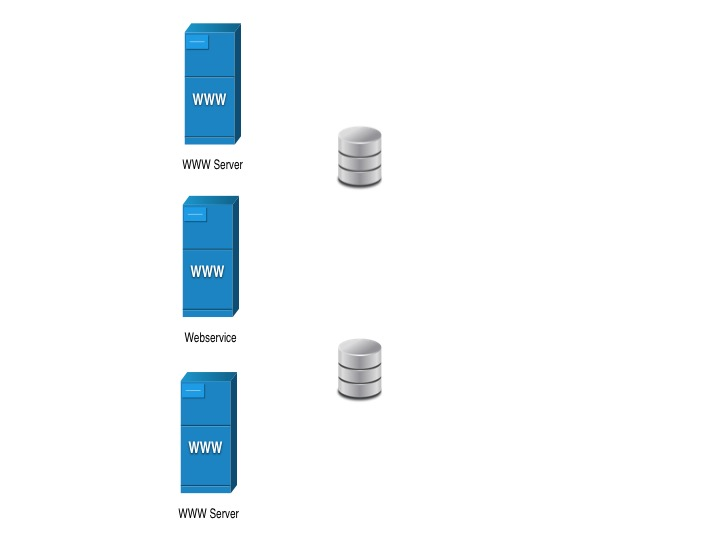
\includegraphics[scale=0.6]{pics/sample-infrastructure-1.eps} \\
\end{center}
\vspace*{\fill}

\subsection{The Job of a System Administrator}
\vspace*{\fill}
\begin{center}
	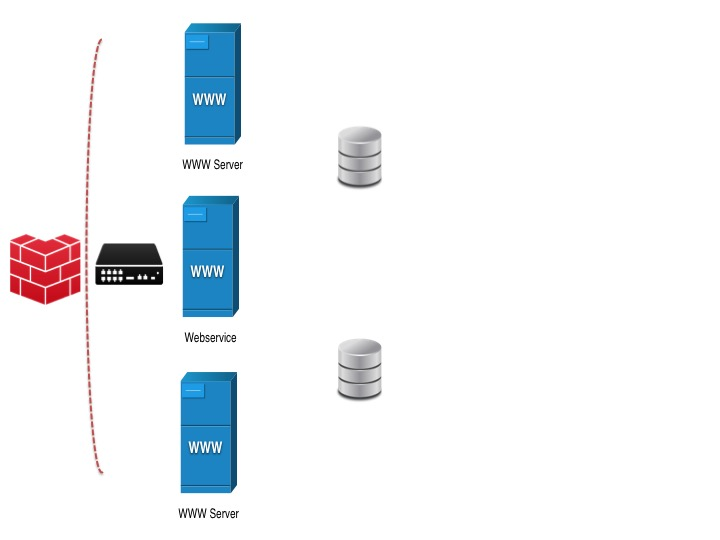
\includegraphics[scale=0.6]{pics/sample-infrastructure-2.eps} \\
\end{center}
\vspace*{\fill}

\subsection{The Job of a System Administrator}
\vspace*{\fill}
\begin{center}
	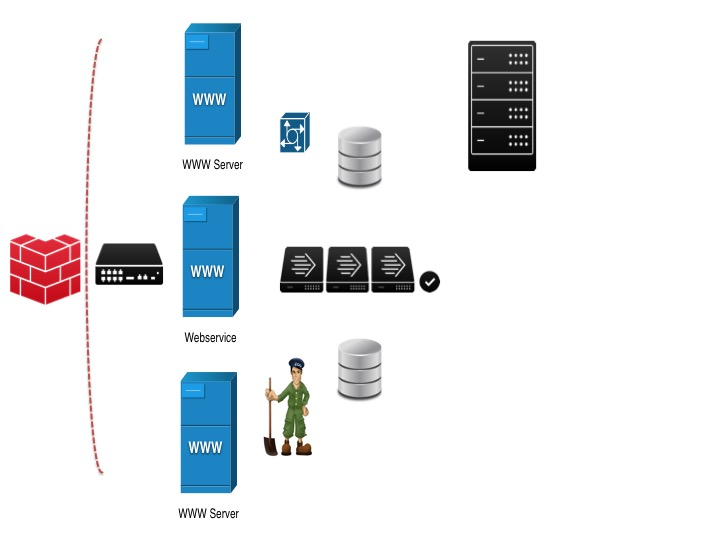
\includegraphics[scale=0.6]{pics/sample-infrastructure-3.eps} \\
\end{center}
\vspace*{\fill}

\subsection{The Job of a System Administrator}
\vspace*{\fill}
\begin{center}
	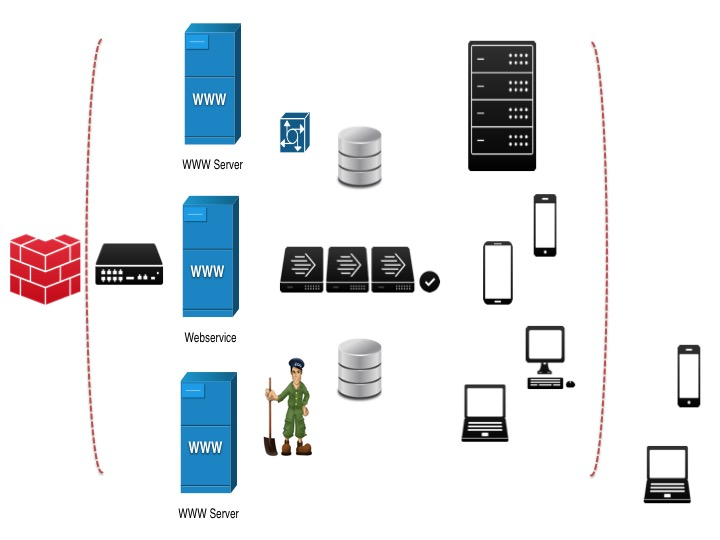
\includegraphics[scale=0.6]{pics/sample-infrastructure-4.eps} \\
\end{center}
\vspace*{\fill}

\subsection{The Job of a System Administrator}
\vspace*{\fill}
\begin{center}
	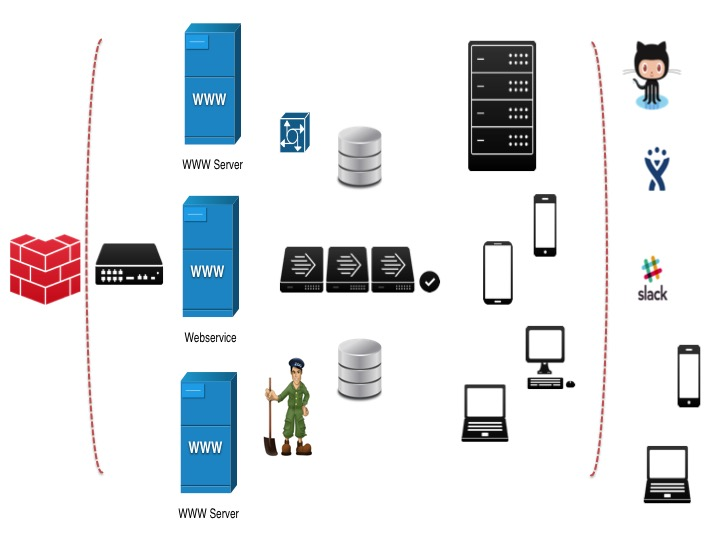
\includegraphics[scale=0.6]{pics/sample-infrastructure-5.eps} \\
\end{center}
\vspace*{\fill}

\subsection{The Job of a System Administrator}
\vspace*{\fill}
\begin{center}
	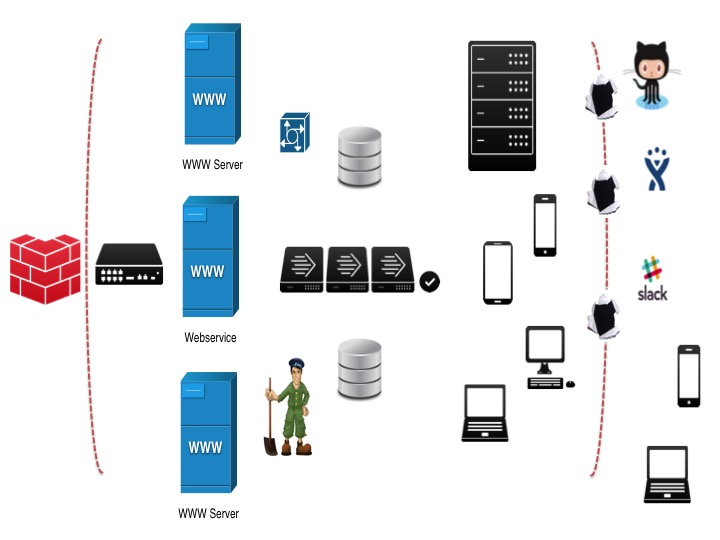
\includegraphics[scale=0.6]{pics/sample-infrastructure-6.eps} \\
\end{center}
\vspace*{\fill}

\subsection{The Job of a System Administrator}
\vspace*{\fill} \begin{center}
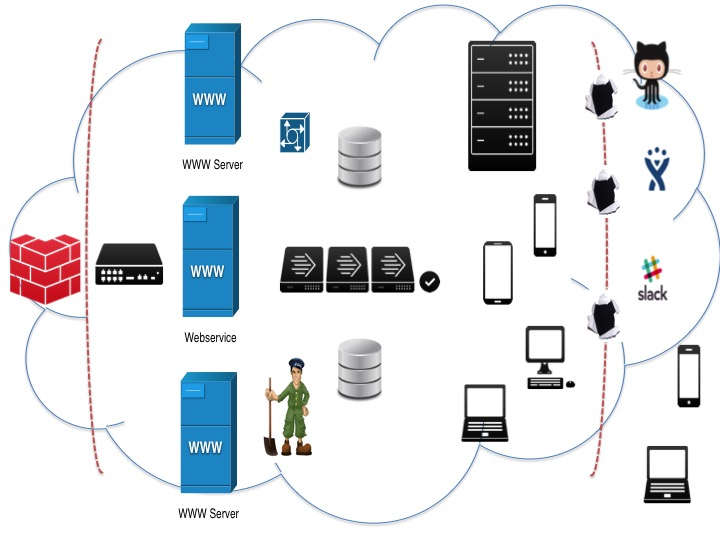
\includegraphics[scale=0.6]{pics/sample-infrastructure-7.eps}
\\ \end{center} \vspace*{\fill}

\subsection{The Job of a System Administrator}
\vspace*{\fill}
\begin{center}
	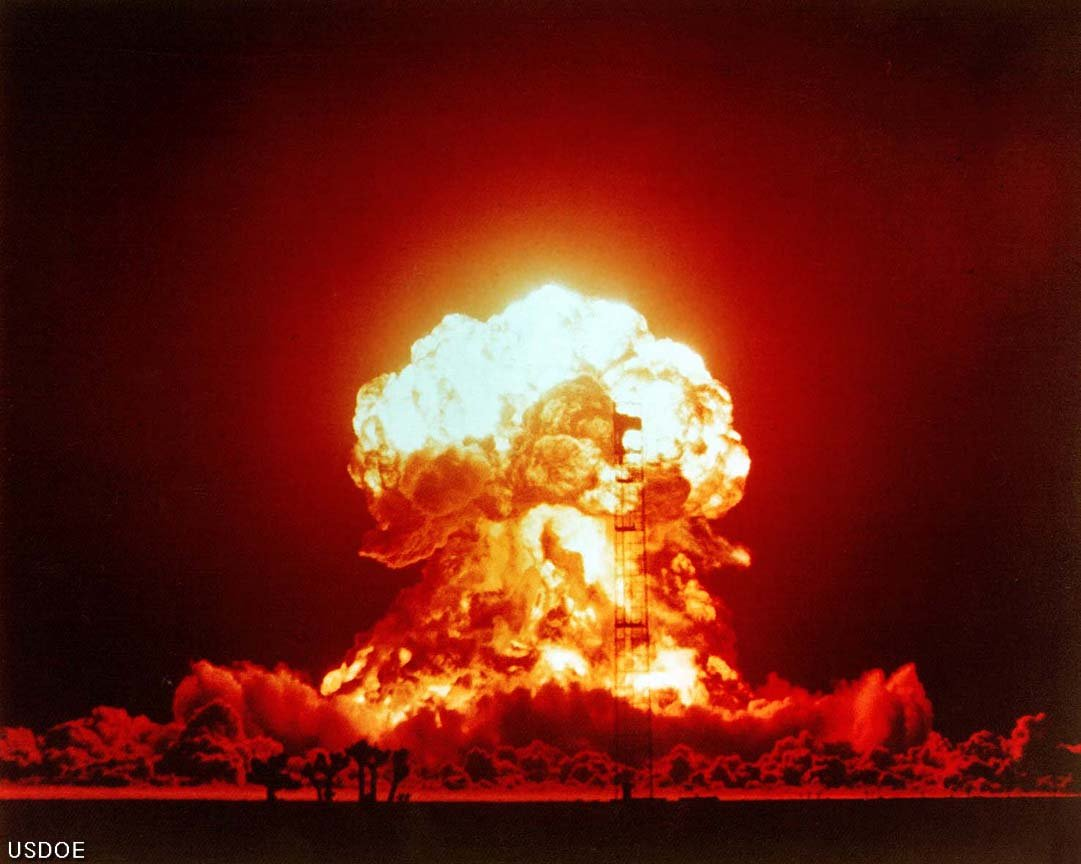
\includegraphics[scale=0.4]{pics/mushroom_cloud.eps} \\
\end{center}
\vspace*{\fill}



\subsection{The Job of a System Administrator}
\vspace*{\fill}
\begin{center}
	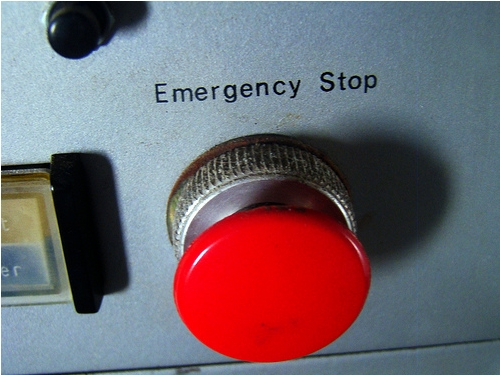
\includegraphics[scale=0.8]{pics/big-red-button.eps} \\
\end{center}
\vspace*{\fill}

\subsection{The Job of a System Administrator}
\vspace*{\fill}
\begin{center}
	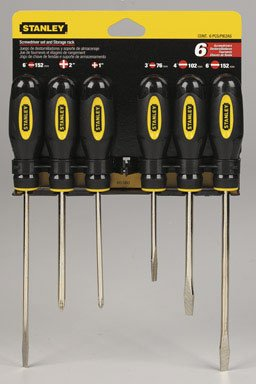
\includegraphics[scale=0.75]{pics/screwdrivers.eps} \\
\end{center}
\vspace*{\fill}

\subsection{The Job of a System Administrator}
\vspace*{\fill}
\begin{center}
	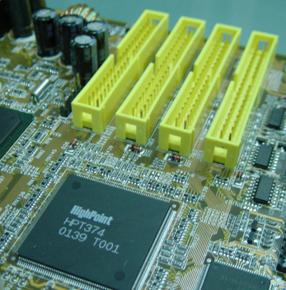
\includegraphics[scale=1.2]{pics/raid.eps} \\
\end{center}
\vspace*{\fill}

\subsection{The Job of a System Administrator}
\vspace*{\fill}
\begin{center}
	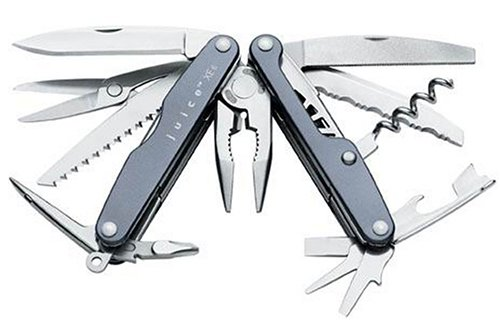
\includegraphics[scale=0.85]{pics/leatherman.eps} \\
\end{center}
\vspace*{\fill}

\subsection{The Job of a System Administrator}
\vspace*{\fill}
\begin{center}
	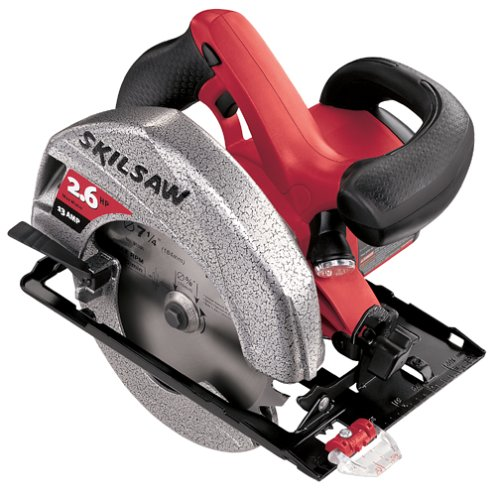
\includegraphics[scale=0.5]{pics/circularsaw.eps} \\
	\small See also: {\tt http://is.gd/WUezLL} \Normalsize
\end{center}
\vspace*{\fill}

\subsection{The Job of a System Administrator}
\vspace*{\fill}
\begin{center}
	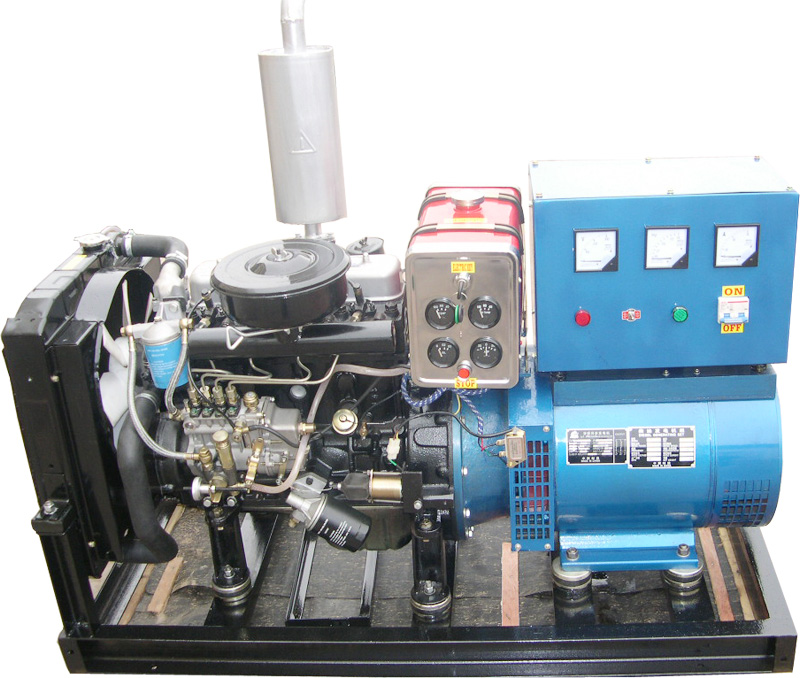
\includegraphics[scale=1.9]{pics/diesel-generator.eps} \\
\end{center}
\vspace*{\fill}

\subsection{The Job of a System Administrator}
\vspace*{\fill}
\begin{center}
	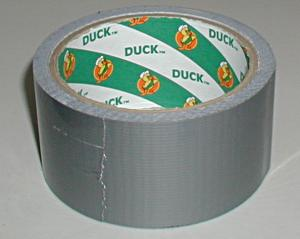
\includegraphics[scale=1.1]{pics/DuckTape.eps} \\
\end{center}
\vspace*{\fill}

\subsection{The Job of a System Administrator}
\vspace*{\fill}
\begin{center}
	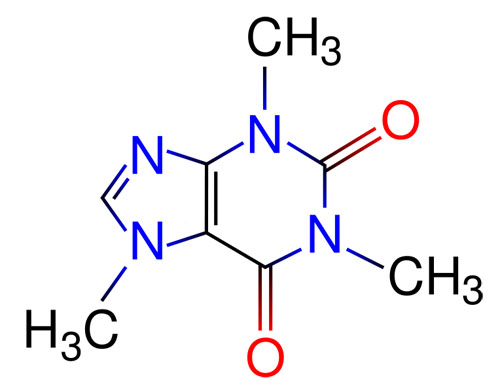
\includegraphics[scale=0.65]{pics/Caffeine_molecule.eps} \\
\end{center}
\vspace*{\fill}

\subsection{The Job of a System Administrator}
\vspace*{\fill}
\begin{center}
	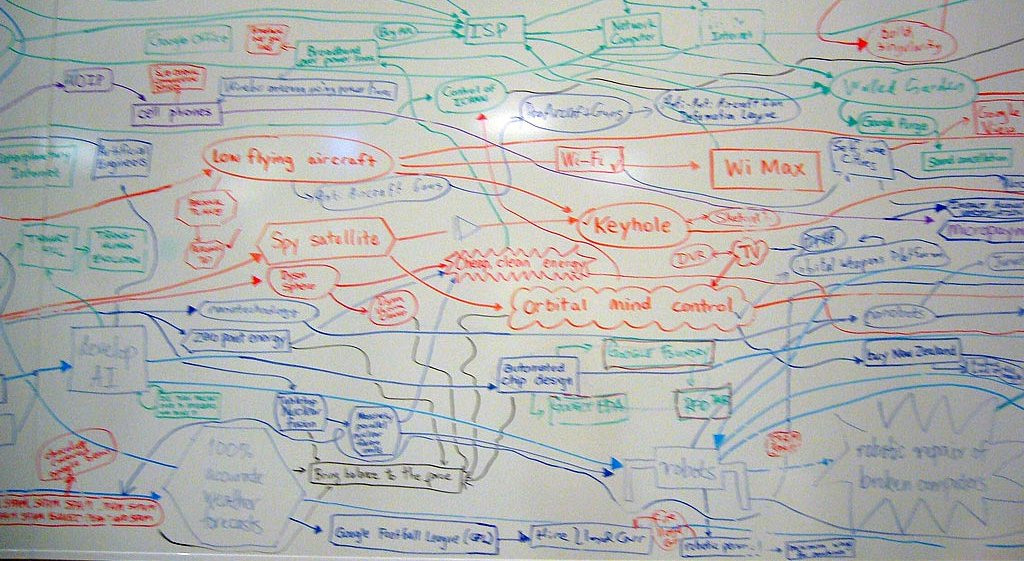
\includegraphics[scale=0.52]{pics/google_whiteboard_large.eps} \\
\end{center}
\vspace*{\fill}

\subsection{The Job of a System Administrator}
\vspace*{\fill}
\begin{center}
	
\includegraphics[scale=0.7]{pics/homer-brain.eps} \\
\end{center}
\vspace*{\fill}

\subsection{The Job of a System Administrator}
What {\bf exactly} does a {\em System Administrator} do?

\subsection{The Job of a System Administrator}
What {\bf exactly} does a {\em System Administrator} do?
\begin{itemize}
	\item no precise job description
\end{itemize}

\subsection{The Job of a System Administrator}
What {\bf exactly} does a {\em System Administrator} do?
\begin{itemize}
	\item no precise job description
\end{itemize}

	\begin{center}
		\includegraphics[scale=1.0]{pics/matrix.eps} \\
	\end{center}




\subsection{The Job of a System Administrator}
What {\bf exactly} does a {\em System Administrator} do?
\begin{itemize}
	\item no precise job description
\end{itemize}
\vfill
 system administrator n.: \\
{\em one who, as a primary job function,
	manages computer and network systems on behalf of another, such as an
	employer or client.}

\subsection{The Job of a System Administrator}
What {\bf exactly} does a {\em System Administrator} do?
\begin{itemize}
	\item no precise job description
	\item often learned by experience
\end{itemize}
\vfill
system administrator n.: \\
{\em one who, as a primary job function,
	manages computer and network systems on behalf of another, such as an
	employer or client.}

\subsection{The Job of a System Administrator}
What {\bf exactly} does a {\em System Administrator} do?
\begin{itemize}
	\item no precise job description
	\item often learned by experience
	\item ``makes things run''
\end{itemize}
\vfill
system administrator n.: \\
{\em one who, as a primary job function,
	manages computer and network systems on behalf of another, such as an
	employer or client.}

\subsection{The Job of a System Administrator}
What {\bf exactly} does a {\em System Administrator} do?
\begin{itemize}
	\item no precise job description
	\item often learned by experience
	\item ``makes things run''
	\item work behind the scenes
\end{itemize}
\vfill
system administrator n.: \\
{\em one who, as a primary job function,
	manages computer and network systems on behalf of another, such as an
	employer or client.}

\subsection{The Job of a System Administrator}
What {\bf exactly} does a {\em System Administrator} do?
\begin{itemize}
	\item no precise job description
	\item often learned by experience
	\item ``makes things run''
	\item work behind the scenes
	\item often known as Operator, Network Administrator, System Programmer, System
		Manager, Service Engineer, Site Reliability Engineer etc.
\end{itemize}
\vfill
system administrator n.: \\
{\em one who, as a primary job function,
	manages computer and network systems on behalf of another, such as an
	employer or client.}

\subsection{So what is a {\em System}?}
``A group of interacting, interrelated, or interdependent elements that
together form a complex whole.''


\subsection{So what is a {\em System}?}
``A group of interacting, interrelated, or interdependent elements that
together form a complex whole.''
\\

In the context of this class, we generally consider {\em computer-human
systems} consisting of

\begin{itemize}
	\item the computer(s)
\end{itemize}

\subsection{So what is a {\em System}?}
``A group of interacting, interrelated, or interdependent elements that
together form a complex whole.''
\\

In the context of this class, we generally consider {\em computer-human
systems} consisting of

\begin{itemize}
	\item the computer(s)
	\item the network
\end{itemize}

\subsection{So what is a {\em System}?}
``A group of interacting, interrelated, or interdependent elements that
together form a complex whole.''
\\

In the context of this class, we generally consider {\em computer-human
systems} consisting of

\begin{itemize}
	\item the computer(s)
	\item the network
\end{itemize}
\vspace{.2in}

\begin{itemize}
	\item the user(s)
\end{itemize}

\subsection{So what is a {\em System}?}
``A group of interacting, interrelated, or interdependent elements that
together form a complex whole.''
\\

In the context of this class, we generally consider {\em computer-human
systems} consisting of

\begin{itemize}
	\item the computer(s)
	\item the network
\end{itemize}
\vspace{.2in}

\begin{itemize}
	\item the user(s)
	\item the organization's goals and policies
\end{itemize}

\subsection{The Job of a System Administrator}
\vspace*{\fill}
\begin{center}
	\includegraphics[scale=0.35]{pics/as-seen-by-not-helping.eps} \\
\end{center}
\vspace*{\fill}

\subsection{The Job of a System Administrator}
\Huge
\vspace*{\fill}
\begin{center}
Computering, at its heart,\\
is a people problem.
\end{center}
\vspace*{\fill}
\Normalsize



\subsection{... and {\em Administration}?}
Merriam Webster:
\begin{quote}
	{\bf administer, v:} {\em to manage or supervise the execution, use, or conduct of} \\
\end{quote}


\subsection{... and {\em Administration}?}
Merriam Webster:
\begin{quote}
	{\bf administer, v:} {\em to manage or supervise the execution, use, or conduct of} \\
\end{quote}

{\em System} Administration frequently also includes other tasks such as
\begin{itemize}
	\item system design and architecture
\end{itemize}

\subsection{... and {\em Administration}?}
Merriam Webster:
\begin{quote}
	{\bf administer, v:} {\em to manage or supervise the execution, use, or conduct of} \\
\end{quote}

{\em System} Administration frequently also includes other tasks such as
\begin{itemize}
	\item system design and architecture
	\item reliability studies
\end{itemize}

\subsection{... and {\em Administration}?}
Merriam Webster:
\begin{quote}
	{\bf administer, v:} {\em to manage or supervise the execution, use, or conduct of} \\
\end{quote}


{\em System} Administration frequently also includes other tasks such as
\begin{itemize}
	\item system design and architecture
	\item reliability studies
	\item resource management
\end{itemize}

\subsection{... and {\em Administration}?}
Merriam Webster:
\begin{quote}
	{\bf administer, v:} {\em to manage or supervise the execution, use, or conduct of} \\
\end{quote}

{\em System} Administration frequently also includes other tasks such as
\begin{itemize}
	\item system design and architecture
	\item reliability studies
	\item resource management
	\item system fault diagnosis
\end{itemize}

\subsection{... and {\em Administration}?} Merriam Webster: \begin{quote} {\bf
administer, v:} {\em to manage or supervise the execution, use, or conduct of}
\\ \end{quote}

{\em System} Administration frequently also includes other tasks such as
\begin{itemize}
	\item system design and architecture
	\item reliability studies
	\item resource management
	\item system fault diagnosis
	\item ...
\end{itemize}


\subsection{... and {\em Administration}?}
Merriam Webster:
\begin{quote}
	{\bf administer, v:} {\em to manage or supervise the execution, use, or conduct of} \\
\end{quote}

{\em System} Administration frequently also includes other tasks such as
\begin{itemize}
	\item system design and architecture
	\item reliability studies
	\item resource management
	\item system fault diagnosis
	\item ...
\end{itemize}
\vspace{.5in}

...all of which my involve a fair amount of {\em software development}, {\em
programming} and {\em scripting}.

\subsection{Learning System Administration}
System Administration is a profession with no fixed career path.

\subsection{Learning System Administration}
System Administration is a profession with no fixed career path.

\begin{itemize}
	\item few degree granting programs
\end{itemize}

\subsection{Learning System Administration}
System Administration is a profession with no fixed career path.

\begin{itemize}
	\item few degree granting programs
	\item heavy reliance on practical experience
\end{itemize}

\subsection{Learning System Administration}
System Administration is a profession with no fixed career path.

\begin{itemize}
	\item few degree granting programs
	\item heavy reliance on practical experience
	\item specializations in many different areas possible
\end{itemize}

\subsection{Learning System Administration}
System Administration is a profession with no fixed career path.

\begin{itemize}
	\item few degree granting programs
	\item heavy reliance on practical experience
	\item specializations in many different areas possible
	\item breadth of expertise as necessary as depth in some areas
\end{itemize}


\subsection{Learning System Administration}
System Administration is a profession with no fixed career path.

\begin{itemize}
	\item few degree granting programs
	\item heavy reliance on practical experience
	\item specializations in many different areas possible
	\item breadth of expertise as necessary as depth in some areas
	\item background knowledge and requirements vary
\end{itemize}

\subsection{Learning System Administration}

Breadth of knowledge:
\begin{itemize}
	\item operating system concepts
	\item TCP/IP networking
	\item programming
	\item ...
\end{itemize}
\vspace{.5in}

Depth of knowledge:
\begin{itemize}
	\item certain OS flavor
	\item specific service (DNS, E-Mail, Databases, Content-Delivery, ...)
	\item specific implementation/vendor (Oracle, Hadoop, Apache, Cisco, ...)
	\item specific are of expertise (security, storage, network, data center, ...)
	\item ...
\end{itemize}

\subsection{People think the internet looks like this.}
\begin{center}
	\includegraphics[scale=0.7]{pics/cloud.eps}
\end{center}

\subsection{Or like this.}
\begin{center}
	\includegraphics[scale=0.4]{pics/internet.eps} \\
	\small
	{\tt http://www.opte.org/maps/}
	\Normalsize
\end{center}

\subsection{SysAdmins know it looks like this.}
\vspace*{\fill}
\begin{center}
    \includegraphics[scale=0.9]{pics/car-duct-tape.eps}
\end{center}
\vspace*{\fill}

\newpage
\vspace*{\fill}
\begin{center}
    \Hugesize
        Hooray! \\ [1em]
    \hspace*{5mm}
    \blueline\\
    \hspace*{5mm}\\
        5 Minute Break
\end{center}
\vspace*{\fill}

\subsection{In reality...}
\vspace*{\fill}
\begin{center}
    \includegraphics[scale=0.9]{pics/car-duct-tape.eps}
\end{center}
\vspace*{\fill}

\subsection{Computer Science}
\vspace*{\fill}
\begin{center}
	\includegraphics[scale=0.6]{pics/CS-venn.eps}
\Normalsize
\end{center}
\vspace*{\fill}

\subsection{About this class}
We can only cover {\em some} of the aspects of System Administration.
\vspace*{\fill}
\begin{center}
	\includegraphics[scale=0.8]{pics/hats.eps}
\Normalsize
\end{center}
\vspace*{\fill}

\subsection{SysAdmins' favorite tool}
\begin{center}
	\includegraphics[scale=1.0]{pics/DuckTape.eps} \\
	\vspace{.5in}
	\small
	\verb+https://www.netmeister.org/blog/duct-tape-and-wd40.html+
	\Normalsize
\end{center}

\subsection{Three Pillars of Exceptional System Design}
We will give particular attention to these three core features:
\begin{itemize}
	\item Scalability
	\item Security
	\item Simplicity
\end{itemize}

\subsection{Three Pillars of Exceptional System Design: Scalability}
\vspace*{\fill}
\begin{center}
    \includegraphics[scale=0.8]{pics/donkey_too_small_for_load.eps} \\
	System Overload
\end{center}
\vspace*{\fill}

\subsection{Three Pillars of Exceptional System Design: Scalability}
\vspace*{\fill}
\begin{center}
    \includegraphics[scale=0.2]{pics/donkey_too_small_for_load.eps} \\
    \includegraphics[scale=0.4]{pics/ardennes-horse.eps} \\
	Scaling Vertically
\end{center}
\vspace*{\fill}


\subsection{Three Pillars of Exceptional System Design: Scalability}
\vspace*{\fill}
\begin{center}
    \includegraphics[scale=0.2]{pics/donkey_too_small_for_load.eps} \\
    \includegraphics[scale=0.5]{pics/vierspaenner.eps} \\
	Scaling Horizontally
\end{center}
\vspace*{\fill}

\subsection{Three Pillars of Exceptional System Design: Scalability}
\vspace*{\fill}
\begin{center}
    \includegraphics[scale=0.2]{pics/donkey_too_small_for_load.eps} \\
    \includegraphics[scale=1.1]{pics/dogcart.eps} \\
	Scaling Down
\end{center}
\vspace*{\fill}

\subsection{Three Pillars of Exceptional System Design: Security}
\vspace*{\fill}
\begin{center}
    \includegraphics[scale=1.4]{pics/usability-security.eps} \\
\end{center}
\vspace*{\fill}

\subsection{Three Pillars of Exceptional System Design: Security}
\vspace*{\fill}
\begin{center}
    \includegraphics[scale=1.4]{pics/chicken-egg.eps} \\
\end{center}
\vspace*{\fill}

\subsection{Three Pillars of Exceptional System Design: Security}
\vspace*{\fill}
\begin{center}
    \includegraphics[scale=0.8]{pics/security-usability.eps} \\
	\small
	{\tt https://www.netmeister.org/blog/infosec-basics.html}
	\Normalsize
\end{center}
\vspace*{\fill}

\subsection{Three Pillars of Exceptional System Design: Simplicity}
\vspace*{\fill}
\begin{center}
    \includegraphics[scale=0.3]{pics/kiss.eps} \\
\end{center}
\vspace*{\fill}

\subsection{Three Pillars of Exceptional System Design: Simplicity}
\vspace*{\fill}
\begin{center}
    \includegraphics[scale=1.2]{pics/lego-block.eps}
\end{center}
\vspace*{\fill}

\subsection{Three Pillars of Exceptional System Design: Simplicity}
\vspace*{\fill}
\begin{center}
    \includegraphics[scale=0.1]{pics/millennium-falcon.eps} \\
\end{center}
\vspace*{\fill}

\subsection{SysAdmins' favorite Laws}
\smallish
Ockham's Razor:
\begin{quote}
{\em ``Of two equivalent theories or explanations, all other things being
equal, the simpler one is to be preferred.''}
\end{quote}
\Normalsize

\subsection{SysAdmins' favorite Laws}
\smallish
Ockham's Razor:
\begin{quote}
{\em ``Of two equivalent theories or explanations, all other things being
equal, the simpler one is to be preferred.''}
\end{quote}

2nd Law of Thermodynamics:
\begin{quote}
{\em ``The entropy of an isolated system always increases with time.''}
\end{quote}
\Normalsize

\subsection{SysAdmins' favorite Laws}
\smallish
Ockham's Razor:
\begin{quote}
{\em ``Of two equivalent theories or explanations, all other things being
equal, the simpler one is to be preferred.''}
\end{quote}

2nd Law of Thermodynamics:
\begin{quote}
{\em ``The entropy of an isolated system always increases with time.''}
\end{quote}

Hanlon's Razor:
\begin{quote}
{\em ``Never attribute to malice that which can be adequately explained by
stupidity.''}
\end{quote}
\Normalsize

\subsection{SysAdmins' favorite Laws}
\smallish
Ockham's Razor:
\begin{quote}
{\em ``Of two equivalent theories or explanations, all other things being
equal, the simpler one is to be preferred.''}
\end{quote}

2nd Law of Thermodynamics:
\begin{quote}
{\em ``The entropy of an isolated system always increases with time.''}
\end{quote}

Hanlon's Razor:
\begin{quote}
{\em ``Never attribute to malice that which can be adequately explained by
stupidity.''}
\end{quote}

Pareto's Principle:
\begin{quote}
{\em ``80\% of consequences stem from 20\% of the causes.''}
\end{quote}
\Normalsize

\subsection{SysAdmins' favorite Laws}
\smallish
Ockham's Razor:
\begin{quote}
{\em ``Of two equivalent theories or explanations, all other things being
equal, the simpler one is to be preferred.''}
\end{quote}

2nd Law of Thermodynamics:
\begin{quote}
{\em ``The entropy of an isolated system always increases with time.''}
\end{quote}

Hanlon's Razor:
\begin{quote}
{\em ``Never attribute to malice that which can be adequately explained by
stupidity.''}
\end{quote}

Pareto's Principle:
\begin{quote}
{\em ``80\% of consequences stem from 20\% of the causes.''}
\end{quote}

Sturgeon's Law:
\begin{quote}
{\em ``90\% of everything is crud.''}
\end{quote}
\Normalsize

\subsection{SysAdmins' favorite Laws}
\smallish
Ockham's Razor:
\begin{quote}
{\em ``Of two equivalent theories or explanations, all other things being
equal, the simpler one is to be preferred.''}
\end{quote}

2nd Law of Thermodynamics:
\begin{quote}
{\em ``The entropy of an isolated system always increases with time.''}
\end{quote}

Hanlon's Razor:
\begin{quote}
{\em ``Never attribute to malice that which can be adequately explained by
stupidity.''}
\end{quote}

Pareto's Principle:
\begin{quote}
{\em ``80\% of consequences stem from 20\% of the causes.''}
\end{quote}

Sturgeon's Law:
\begin{quote}
{\em ``90\% of everything is crud.''}
\end{quote}

Murphy's Law:
\begin{quote}
{\em ``If it can happen, it will happen.''}
\end{quote}
\Normalsize


\subsection{SysAdmins' favorite Laws}
\smallish
Ockham's Razor:
\begin{quote}
{\em ``Of two equivalent theories or explanations, all other things being
equal, the simpler one is to be preferred.''}
\end{quote}

2nd Law of Thermodynamics:
\begin{quote}
{\em ``The entropy of an isolated system always increases with time.''}
\end{quote}

Hanlon's Razor:
\begin{quote}
{\em ``Never attribute to malice that which can be adequately explained by
stupidity.''}
\end{quote}

Pareto's Principle:
\begin{quote}
{\em ``80\% of consequences stem from 20\% of the causes.''}
\end{quote}

Sturgeon's Law:
\begin{quote}
{\em ``90\% of everything is crud.''}
\end{quote}

Murphy's Law:
\begin{quote}
{\em ``If it can happen, it will happen.''}
\end{quote}

Throw in some philosophy for good measure:
\begin{quote}
{\em Causality: For every effect, there must be a cause.}
\end{quote}
\Normalsize

\subsection{Learning is critical}
Know how to find answers:
\begin{itemize}
	\item know {\em how} to ask questions
	\item know {\em where} to ask questions
	\item read critically
	\item know what you don't know (Dunning-Kruger effect)
	\item understand {\em what} you're doing
	\item understand {\em why} you're doing it
	\item seek information exchange
\end{itemize}

\subsection{Learning is critical}
\vspace{1in}
\Huge
\begin{center}
``Computer Science projects are opportunities, \\
not assignments.'' \\
\end{center}
\Normalsize

\subsection{Learning is critical}
Know how to find answers:
\begin{itemize}
	\item know {\em how} to ask questions
	\item know {\em where} to ask questions
	\item read critically
	\item know what you don't know (Dunning-Kruger effect)
	\item understand {\em what} you're doing
	\item understand {\em why} you're doing it
	\item seek information exchange
\end{itemize}
\vspace{.5in}
\verb+https://www.cs.stevens.edu/~jschauma/615/meetup.html+

\subsection{Syllabus}
Dates and Topics subject to change:
\begin{itemize}
	\item 01/22: Introduction, UNIX history and basics
	\item 01/29: Filesystems and Disks
	\item 02/05: Software Installation Concepts
	\item 02/12: Multi-user basics
	\item 02/21 - 02/26: Networking
	\item 03/05 - 03/19: DNS, HTTP, HTTPS, Monitoring
	\item 03/26: Writing System Tools
	\item 04/02: SMTP; Backup and Disaster Recovery
	\item 04/09: Configuration Management
	\item 04/16: Ethics and Social Responsibility
	\item 04/23: System Security
\end{itemize}

\subsection{About this class}
No textbook, but plenty of recommended reading materials. \\

Mandatory pre-class surveys. \\

Grading:
\begin{itemize}
	\item course participation, course notes
	\item homework assignments
	\item group project(s)
	\item {\em no curve}
	\item {\em no late submissions}
	\item {\em no extra credit}
	\item {\em no make-up assignments}
\end{itemize}

\verb+https://lists.stevens.edu/mailman/listinfo/cs615asa+

\subsection{Course Notes}
\begin{itemize}
	\item create a git repository with a single text file for each lecture
	\item before each lecture, note:
		\begin{itemize}
			\item what you read
			\item what questions you have
		\end{itemize}
	\item after each lecture:
		\begin{itemize}
			\item answers you've found, or especially interesting new things you learned
			\item what questions remain
			\item what new questions arose
			\item what additional reading might be relevant
		\end{itemize}
	\item share
	\item at the end of the semester, submit all your notes
\end{itemize}

\verb+https://www.cs.stevens.edu/~jschauma/615/course-notes.html+

\pagebreak

\vspace*{\fill}
\begin{center}
  \Hugesize
    UNIX History
	\hspace*{5mm}\blueline\\ [1em]
  \Normalsize
\end{center}
\vspace*{\fill}

\subsection{UNIX history}
\verb+http://www.unix.org/what_is_unix/history_timeline.html+ \\

\begin{itemize}
	\item Originally developed in 1969 at Bell Labs by Ken Thompson
		and Dennis Ritchie.
	\item 1973, Rewritten in C. This made it portable and changed the history of OS
	\item 1974: Thompson, Joy, Haley and students at Berkeley develop
		the {\bf B}erkeley {\bf S}oftware {\bf D}istribution (BSD) of UNIX
	\item two main directions emerge: BSD and what was to become ``System V''
\end{itemize}

\subsection{Notable dates in UNIX history}
\begin{itemize}
	\item 1984 4.2BSD released (TCP/IP), 1986 4.3BSD released (NFS)
	\item 1991 Linus Torvalds starts working on the Linux kernel
	\item 1993 Settlement of USL vs. BSDi; NetBSD, then FreeBSD are created
	\item 1994 Single UNIX Specification introduced
	\item 1995 4.4BSD-Lite Release 2 (last CSRG release); OpenBSD
		forked off NetBSD
	\item 2000 Darwin created (derived from NeXT, FreeBSD, NetBSD)
	\item 2003 Xen; SELinux
	\item 2005 Hadoop; DTrace; ZFS; Solaris Containers
	\item 2006 AWS ("Cloud Computing" comes full circle)
	\item 2007 iOS; KVM appears in Linux
	\item 2008 Android; Solaris open sourced as OpenSolaris
\end{itemize}

\subsection{Some UNIX versions}
More UNIX (some generic, some trademark, some just unix-like):
\\

\small
\begin{tabular}{ c c c c c}
	1BSD & 2BSD & 3BSD & 4BSD & 4.4BSD Lite 1 \\
	4.4BSD Lite 2 & 386 BSD & A/UX & Acorn RISC iX & AIX \\
	AIX PS/2 & AIX/370 & AIX/6000 & AIX/ESA & AIX/RT \\
	AMiX & AOS Lite & AOS Reno & ArchBSD & ASV \\
	Atari Unix & BOS & BRL Unix & BSD Net/1 & BSD Net/2 \\
	BSD/386 & BSD/OS & CB Unix & Chorus & Chorus/MiX \\
	Coherent & CTIX & Darwin & Debian GNU/Hurd & DEC OSF/1 ACP \\
	Digital Unix & DragonFly BSD & Dynix & Dynix/ptx & ekkoBSD \\
	FreeBSD & GNU & GNU-Darwin & HPBSD & HP-UX \\
	HP-UX BLS & IBM AOS & IBM IX/370 & Interactive 386/ix & Interactive IS \\
	IRIX & Linux & Lites & LSX & Mac OS X \\
	Mac OS X Server & Mach & MERT & MicroBSD & Mini Unix \\
	Minix & Minix-VMD & MIPS OS & MirBSD & Mk Linux \\
	Monterey & more/BSD & mt Xinu & MVS/ESA OpenEdition & NetBSD \\
	NeXTSTEP & NonStop-UX & Open Desktop & Open UNIX & OpenBSD \\
	OpenServer & OPENSTEP & OS/390 OpenEdition & OS/390 Unix & OSF/1 \\
	PC/IX & Plan 9 & PWB & PWB/UNIX & QNX \\
	QNX RTOS & QNX/Neutrino & QUNIX & ReliantUnix & Rhapsody \\
	RISC iX & RT & SCO UNIX & SCO UnixWare & SCO Xenix \\
	SCO Xenix System V/386 & Security-Enhanced Linux & Sinix &
		Sinix ReliantUnix & Solaris \\
	SPIX & SunOS & Tru64 Unix & Trusted IRIX/B & Trusted Solaris \\
	Trusted Xenix & TS & UCLA Locus & UCLA Secure Unix & Ultrix \\
	Ultrix 32M & Ultrix-11 & Unicos & Unicos/mk & Unicox-max \\
	UNICS & UNIX 32V & UNIX Interactive & UNIX System III & UNIX System IV \\
	UNIX System V & UNIX System V Release 2 & UNIX System V Release 3 &
		UNIX System V Release 4 & UNIX System V/286 \\
	UNIX System V/386 & UNIX Time-Sharing System & UnixWare & UNSW & USG \\
	Venix & Wollogong & Xenix OS & Xinu & xMach \\
\end{tabular}
\Normalsize

\subsection{UNIX Everywhere}
\Hugesize
\vspace*{\fill}
\begin{center}
Today, your desktop, server, cloud, TV, phone, watch, stereo, car
navigation system, thermostat, door lock, etc. all run a Unix-like OS... \\
\end{center}
\vspace*{\fill}
\Normalsize

\subsection{UNIX Everywhere}
\Hugesize
\vspace*{\fill}
\begin{center}
Today, your desktop, server, cloud, TV, phone, watch, stereo, car
navigation system, thermostat, door lock, etc. all run a Unix-like OS... \\
\vspace{.5in}
...with all the risks that entails.
\end{center}
\vspace*{\fill}
\Normalsize

\pagebreak

\vspace*{\fill}
\begin{center}
  \Hugesize
    UNIX Basics
	\hspace*{5mm}\blueline\\ [1em]
  \Normalsize
\end{center}
\vspace*{\fill}

\subsection{UNIX Basics}
The OS is divided into
\begin{itemize}
	\item kernel
	\item shell
	\item tools \& applications
\end{itemize}
\addvspace{.5in}
Basic UNIX features:
\begin{itemize}
	\item multitasking
	\item multiuser
	\item portability
	\item networking capabilities
\end{itemize}

\subsection{UNIX Basics}
These features necessitate/result in:
\begin{itemize}
	\item multi-user concepts
		\begin{itemize}
			\item user privileges
			\item file permissions
			\item process ownership and priorities
			\item disk quotas
		\end{itemize}
	\item security considerations
		\begin{itemize}
			\item protect users' data
			\item protect communication
			\item protect superuser account
		\end{itemize}
\end{itemize}

\subsection{UNIX Basics: Pipelines}
What is the longest word found on the ten most
frequently retrieved English Wikipedia pages?
\begin{verbatim}
for f in $(curl -L http://is.gd/c6F2fs | zgrep -i "^en " |
        sort -k3 -n | tail -10 |
        sed -e 's/en \(.*\) [0-9]* [0-9]*/\1/'); do
        links -dump http://en.wikipedia.org/wiki/${f}
done |
tr '[:punct:]' ' ' |
tr '[:space:]' '\n' |
tr '[:upper:]' '[:lower:]' |
egrep '^[a-z]+$' |
awk '{ print length() " " $0; }' |
sort |
uniq |
sort -n |
tail -1
\end{verbatim}

\subsection{Program Design}
\verb+https://en.wikipedia.org/wiki/Unix_philosophy+ \\

UNIX programs...
\begin{itemize}
	\item ...are simple
	\item ...follow the element of least surprise
	\item ...accept input from {\tt stdin}
	\item ...generate output to {\tt stdout}
	\item ...generate meaningful error messages to {\tt stderr}
	\item ...have meaningful exit codes
	\item ...have a manual page
\end{itemize}

\subsection{HW}
Make sure you have:
\begin{itemize}
	\item an account on {\tt linux-lab.cs.stevens.edu}
	\item an AWS account
	\item bookmarked the course website
	\item subscribed to the class mailing list
	\item started your course notes
\end{itemize}

\vspace*{\fill}
{\tt https://www.cs.stevens.edu/\~{}jschauma/615/course-notes.html} \\
{\tt https://www.cs.stevens.edu/\~{}jschauma/615/s18-hw1.html} \\
{\tt https://www.cs.stevens.edu/\~{}jschauma/cgi-bin/CS615-02.cgi} \\
\vspace*{\fill}



%\vspace{.5in}
%
%Running an instance:
%\begin{verbatim}
%$ aws ec2 run-instances --key-name stevens --security-groups stevens \
%        --image-id <AMI-ID>
%\end{verbatim}
%
%\subsection{Let's review HW1}
%{\tt http://www.cs.stevens.edu/\~{}jschauma/615/s15-hw1.html} \\
%\vspace{.5in}
%
%Save yourself some typing:
%\begin{verbatim}
%$ alias instance='aws ec2 run-instances --key-name stevens \
%                        --security-groups stevens --image-id'
%$ instance <AMI-ID>
%\end{verbatim}
%
%\subsection{Let's review HW1}
%{\tt http://www.cs.stevens.edu/\~{}jschauma/615/s15-hw1.html} \\
%\vspace{.5in}
%
%
%Make it permanent:
%\begin{verbatim}
%$ echo "alias instance='aws ec2 run-instances --key-name stevens \
%        --security-groups stevens --image-id'" >> .bashrc
%\end{verbatim}
%
%
%\subsection{Let's review HW1}
%{\tt http://www.cs.stevens.edu/\~{}jschauma/615/s15-hw1.html} \\
%\vspace{.5in}
%
%ssh to an instance:
%\begin{verbatim}
%$ ssh -i ~/.ec2/stevens.pem root@<mumble>.compute-1.amazonaws.com
%\end{verbatim}
%
%
%\subsection{Let's review HW1}
%{\tt http://www.cs.stevens.edu/\~{}jschauma/615/s15-hw1.html} \\
%\vspace{.5in}
%
%Let's save ourselves some typing:
%\begin{verbatim}
%$ cat >>~/.ssh/config <<EOF
%> Host *.amazonaws.com
%>         IdentityFile ~/.ec2/stevens.pem
%>         User         root
%> EOF
%$ ssh <mumble>.compute-1.amazonaws.com
%\end{verbatim}
%
%
%\subsection{Filesystems, Disk, Storage}
%\begin{verbatim}
%$ instance ami-35eb835c
%[...]
%$ aws ec2 describe-instances
%[...]
%$ ssh root@ec2-54-198-235-45.compute-1.amazonaws.com
%\end{verbatim}
%
%\subsection{Let's review HW1}
%\begin{verbatim}
%# uname -a
%SunOS domU-12-31-39-0F-1C-BB.compute-1.internal 5.11 omnios-33fdde4 i86pc
%i386 i86xpv Solaris
%#
%\end{verbatim}
%
%\subsection{Let's review HW1}
%\begin{verbatim}
%# ifconfig -a
%lo0: flags=2001000849<UP,LOOPBACK,RUNNING,MULTICAST,IPv4,VIRTUAL> mtu 8232 index 1
%        inet 127.0.0.1 netmask ff000000
%xnf0: flags=1004843<UP,BROADCAST,RUNNING,MULTICAST,DHCP,IPv4> mtu 1500 index 2
%        inet 10.110.94.225 netmask fffffe00 broadcast 10.110.95.255
%        ether 12:31:39:1c:60:13
%lo0: flags=2002000849<UP,LOOPBACK,RUNNING,MULTICAST,IPv6,VIRTUAL> mtu 8252 index 1
%        inet6 ::1/128
%xnf0: flags=20002000840<RUNNING,MULTICAST,IPv6> mtu 1500 index 2
%        inet6 ::/0
%        ether 12:31:39:1c:60:13
%#
%\end{verbatim}
%
%
%\subsection{Let's review HW1}
%\begin{verbatim}
%# netstat -na | more
%[...]
%TCP: IPv4
%   Local Address        Remote Address    Swind Send-Q Rwind Recv-Q
%State
%-------------------- -------------------- ----- ------ ----- ------ -----------
%127.0.0.1.4999             *.*                0      0 128000      0 LISTEN
%      *.111                *.*                0      0 128000      0 LISTEN
%      *.*                  *.*                0      0 128000      0 IDLE
%      *.111                *.*                0      0 128000      0 LISTEN
%      *.*                  *.*                0      0 128000      0 IDLE
%      *.46457              *.*                0      0 128000      0 LISTEN
%      *.55986              *.*                0      0 128000      0 LISTEN
%      *.22                 *.*                0      0 128000      0 LISTEN
%10.110.94.225.22     155.246.89.107.46137 42304     47 128592      0 ESTABLISHED
%[...]
%\end{verbatim}
%
%\subsection{Let's review HW1}
%\begin{verbatim}
%# man df
%[...]
%# df
%[...]
%# df -hT
%[...]
%# df -i
%[...]
%# df -a
%[...]
%# mount
%[...]
%\end{verbatim}
%
%
%\subsection{Let's review HW1}
%\begin{verbatim}
%# format
%[...]
%format> verify
%[...]
%# zpool list
%[...]
%# zfs list
%[...]
%\end{verbatim}
%
\newpage
\vspace*{\fill}
\begin{center}
    \Hugesize
        The End \\ [1em]
    \hspace*{5mm}
    \blueline\\
    \hspace*{5mm}\\
        Hooray!
\end{center}
\vspace*{\fill}

\subsection{Reading}
Miscellaneous:
\begin{itemize}
	\item \verb+http://www.opsschool.org/+
	\item \verb+http://nixsrv.com/llthw+
	\item \verb+http://linuxcommand.org/lc3_learning_the_shell.php+
	\item \verb+http://is.gd/NNAIIm+
\end{itemize}

UNIX history:
\begin{itemize}
	\item \verb+https://www.bell-labs.com/usr/dmr/www/+
	\item \verb+https://www.bell-labs.com/usr/dmr/www/hist.html+
	\item \verb+http://www.futuretech.blinkenlights.nl/admin/day1a.html+
	\item \verb+http://www.levenez.com/unix/+
	\item \verb+https://en.wikipedia.org/wiki/Operating_system+
\end{itemize}

\subsection{Reading}
UNIX basics:
\begin{itemize}
	\item chmod(1), chown(1), ls(1)
	\item intro(1), login(1), passwd(5)
	\item su(1), sudo(8)
\end{itemize}

%\nocite{*}
%\bibliographystyle{plain}
%\bibliography{slides}

\end{document}
